\chapter{Results}\label{ch:results}

This chapter presents the experimental results of different DIP-based denoising approaches.
We first evaluate these methods on standard image datasets, providing a controlled setting for method comparison.
Then, we apply these approaches to DAS data demonstrating its performance in a more complex real-world scenario.

\section{Image Data}

Since clean reference samples are not available for DAS data, we begin by conducting experiments on standard image denoising tasks.
These preliminary evaluations enable a controlled comparison of different methods and configurations.

For all variants, we follow the original DIP paper and set the maximum number of iterations to 2000.
For ES-based methods, we employ the ES-WMV criterion with a patience of 500 iterations.
For DIP-TV, we set $\lambda = 0.1$, and for SG-DIP, we set the number of different noise samples per iteration to 3, as recommended in the original paper.
For SGR-DIP, we linearly increase $\lambda$ from 1 to 10 throughout training. 
As discussed in Section~\ref{sec:architecture}, we use ECA in the skip connections because it tends to retain more fine-grained details, while yielding almost identical performance, as shown in Table~\ref{tab:ECA}. 

\begin{table}
    \small
    \centering
    \begin{tabular}{ l l c c }
        \toprule
        Skip Type &Method &PSNR (dB) $\uparrow$ &SSIM $\in [0,1]$ $\uparrow$ \\
        \midrule
        \multirow{2}{4em}{Conv} &SG-DIP (ES) &26.03 {\scriptsize (2.15)} &0.68 {\scriptsize (0.11)} \\
        &SGR-DIP &\underline{26.34} {\scriptsize (2.12)} &\textbf{0.70} {\scriptsize (0.11)} \\
        \midrule
        \multirow{2}{4em}{ECA} &SG-DIP (ES) &25.97 {\scriptsize (1.92)} &0.68 {\scriptsize (0.11)} \\
        &SGR-DIP &\textbf{26.37} {\scriptsize (2.04)} &\textbf{0.70} {\scriptsize (0.11)} \\
        \bottomrule
    \end{tabular}
    \caption{
        Comparison of different types of skip connections on the Set14 dataset.
        Noisy input images are generated at a PSNR of 15\,dB.
        Values represent mean and {\scriptsize (standard deviation)}.
    }\label{tab:ECA}
\end{table}

We conduct a series of experiments to evaluate the performance of different approaches.

First, we compare the methods on the Set14 dataset at both low and high noise levels.
At low noise levels, all variants --- except for DDIP --- achieve satisfactory results.
However, at high noise levels, explicit regularization becomes crucial, as overfitting occurs very early in the optimization process (see Figure~\ref{fig:noise-levels}).
Among the tested methods, only the ES-based methods and our SGR-DIP are robust across different noise levels, with DIP-TV with ES being the most consistent (see Table~\ref{tab:noise-levels}).

We further evaluate the variants on the CBSD68 dataset with moderate noise added.
While our approach yields the best results, it takes significantly longer to run compared to other methods.
The best tradeoff between denoising performance and runtime is achieved by DIP-TV with ES, as shown in Table~\ref{tab:CBSD68}.
However, in terms of visual quality, it is clearly outperformed by our SGR-DIP, as demonstrated in Figure~\ref{fig:CBSD68}.

\begin{table}
    \small
    \centering
    \begin{tabular}{ l c c c c }
        \toprule
        &\multicolumn{2}{c}{20\,dB} &\multicolumn{2}{c}{10\,dB}\\
        \midrule
        Method &PSNR (dB) $\uparrow$ &SSIM $\in [0,1]$ $\uparrow$ &PSNR (dB) $\uparrow$ &SSIM $\in [0,1]$ $\uparrow$\\
        \midrule
        DIP &27.52 {\scriptsize (1.20)} &0.74 {\scriptsize (0.04)} &16.02 {\scriptsize (0.45)} &0.21 {\scriptsize (0.06)} \\
        DIP (ES) &27.10 {\scriptsize (1.72)} &0.73 {\scriptsize (0.09)} &22.52 {\scriptsize (1.58)} &0.48 {\scriptsize (0.05)} \\
        DIP-TV &28.29 {\scriptsize (2.31)} &\textbf{0.79} {\scriptsize (0.06)} &18.99 {\scriptsize (0.52)} &0.33 {\scriptsize (0.07)} \\
        DIP-TV (ES) &\underline{28.37} {\scriptsize (2.31)} &0.78 {\scriptsize (0.06)} &\underline{23.44} {\scriptsize (1.67)} &\textbf{0.56} {\scriptsize (0.08)} \\
        DDIP &23.15 {\scriptsize (2.84)} &0.58 {\scriptsize (0.14)} &22.58 {\scriptsize (2.57)} &0.54 {\scriptsize (0.10)} \\
        SG-DIP &\textbf{28.50} {\scriptsize (1.97)} &\textbf{0.79} {\scriptsize (0.07)} &12.34 {\scriptsize (1.16)} &0.12 {\scriptsize (0.05)} \\
        SG-DIP (ES) &27.42 {\scriptsize (2.40)} &0.75 {\scriptsize (0.09)} &\textbf{23.49} {\scriptsize (2.16)} &0.54 {\scriptsize (0.10)} \\
        SGR-DIP &26.99 {\scriptsize (2.36)} &0.73 {\scriptsize (0.13)} &23.29 {\scriptsize (2.48)} &\textbf{0.56} {\scriptsize (0.12)} \\
        \bottomrule
    \end{tabular}
    \caption{
        Quantitative comparison of DIP variants on the Set14 dataset at different noise levels.
        Noisy input images are generated at PSNRs of 20\,dB and 10\,dB, respectively.
        Values represent mean and {\scriptsize (standard deviation)}.
    }\label{tab:noise-levels}
\end{table}

\begin{figure}
    \centering
    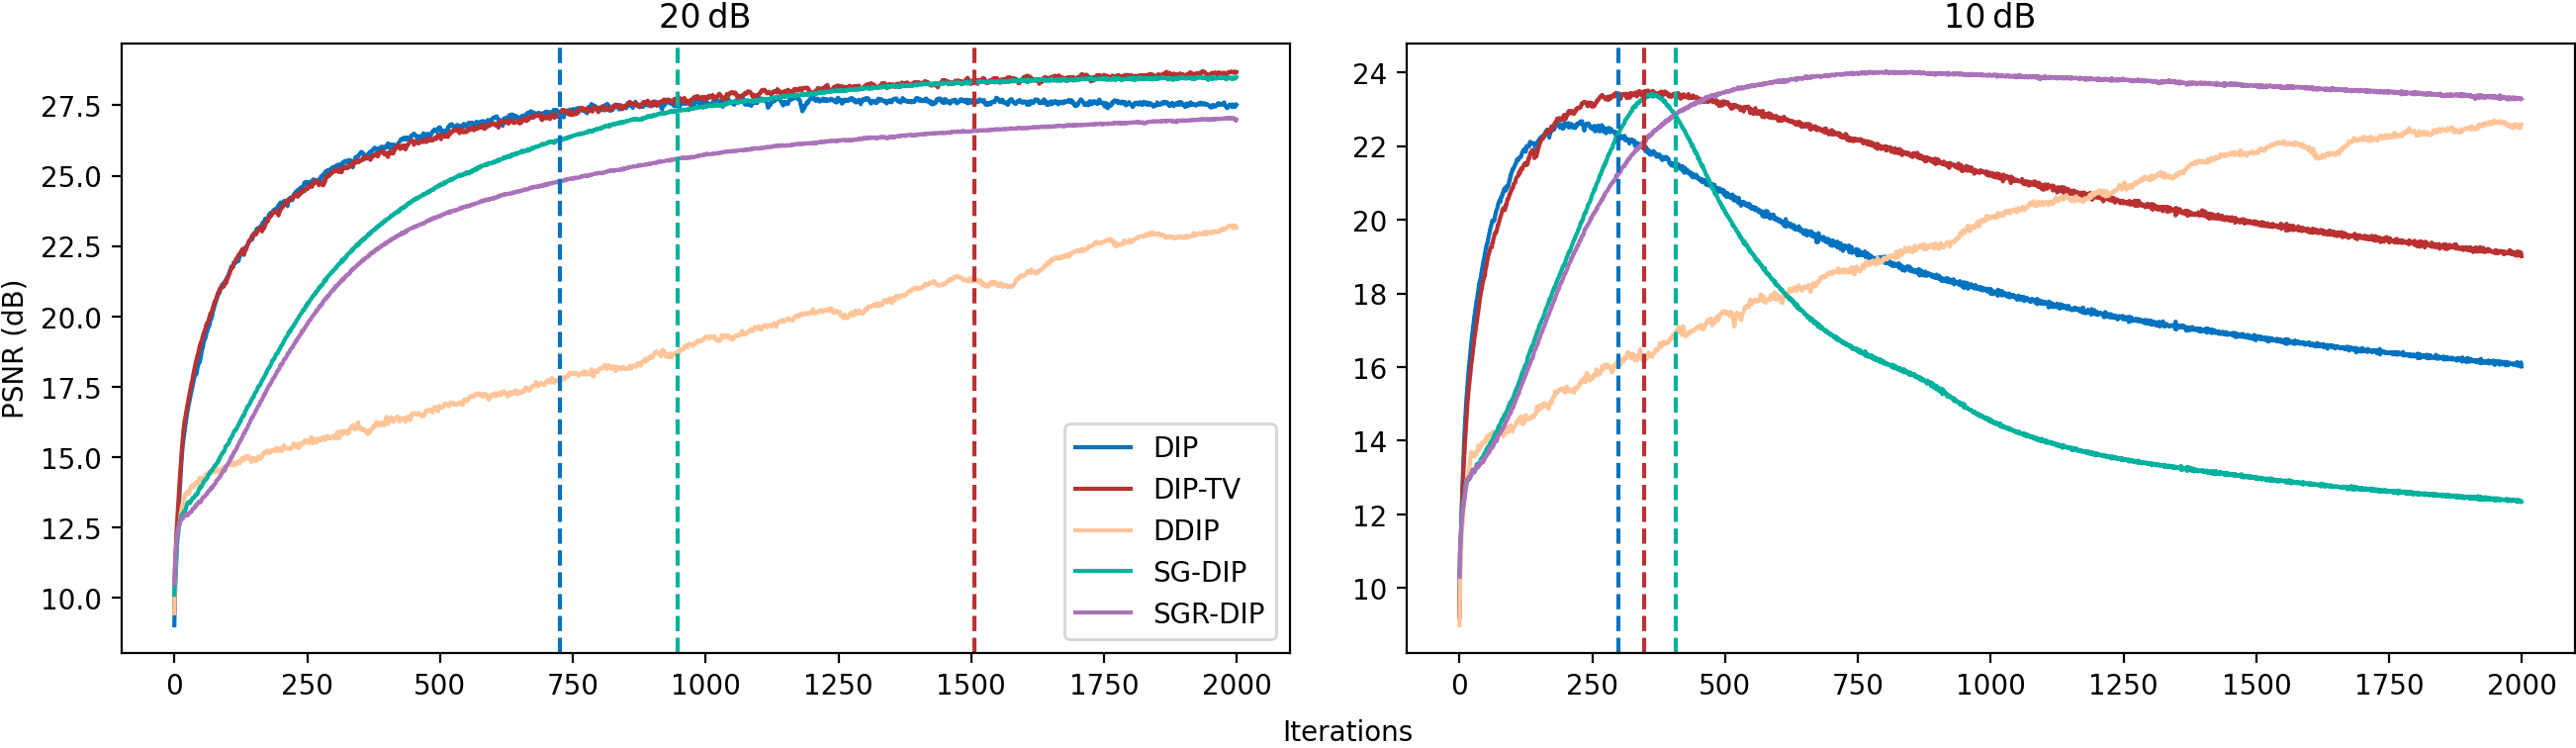
\includegraphics[width=\textwidth]{img/fig_6.1.png}
    \caption{
        Mean PSNR curves of DIP variants on the Set14 dataset at different noise levels.
        Noisy input images are generated at PSNRs of 20\,dB and 10\,dB, respectively.
        Dashed lines represent the average detected stopping points for the corresponding ES-based methods.
    }\label{fig:noise-levels}
\end{figure}

\begin{table}
    \small
    \centering
    \begin{tabular}{ l c c c }
        \toprule
        Method &PSNR (dB) $\uparrow$ &SSIM $\in [0,1]$ $\uparrow$ &Runtime (m) $\downarrow$\\
        \midrule
        DIP &22.32 {\scriptsize (0.74)} &0.43 {\scriptsize (0.11)} &1.31 {\scriptsize (0.01)} \\
        DIP (ES) &25.64 {\scriptsize (2.07)} &0.62 {\scriptsize (0.07)} &\textbf{0.50} {\scriptsize (0.08)} \\
        DIP-TV &26.06 {\scriptsize (1.37)} &0.65 {\scriptsize (0.07)} &1.45 {\scriptsize (0.01)} \\
        DIP-TV (ES) &\underline{26.65} {\scriptsize (2.45)} &\underline{0.69} {\scriptsize (0.10)} &\underline{0.67} {\scriptsize (0.16)} \\
        DDIP &24.54 {\scriptsize (3.15)} &0.61 {\scriptsize (0.13)} &1.34 {\scriptsize (0.01)} \\
        SG-DIP &22.24 {\scriptsize (3.88)} &0.45 {\scriptsize (0.09)} &3.33 {\scriptsize (0.02)} \\
        SG-DIP (ES) &26.57 {\scriptsize (2.47)} &\underline{0.69} {\scriptsize (0.09)} &2.05 {\scriptsize (0.61)} \\
        SGR-DIP &\textbf{26.76} {\scriptsize (2.51)} &\textbf{0.70} {\scriptsize (0.10)} &3.34 {\scriptsize (0.09)} \\
        \bottomrule
    \end{tabular}
    \caption{
        Quantitative comparison of DIP variants on the CBSD68 dataset.
        Noisy input images are generated at a PSNR of 15\,dB.
        Values represent mean and {\scriptsize (standard deviation)}.
    }\label{tab:CBSD68}
\end{table}

\begin{figure}
    \centering
    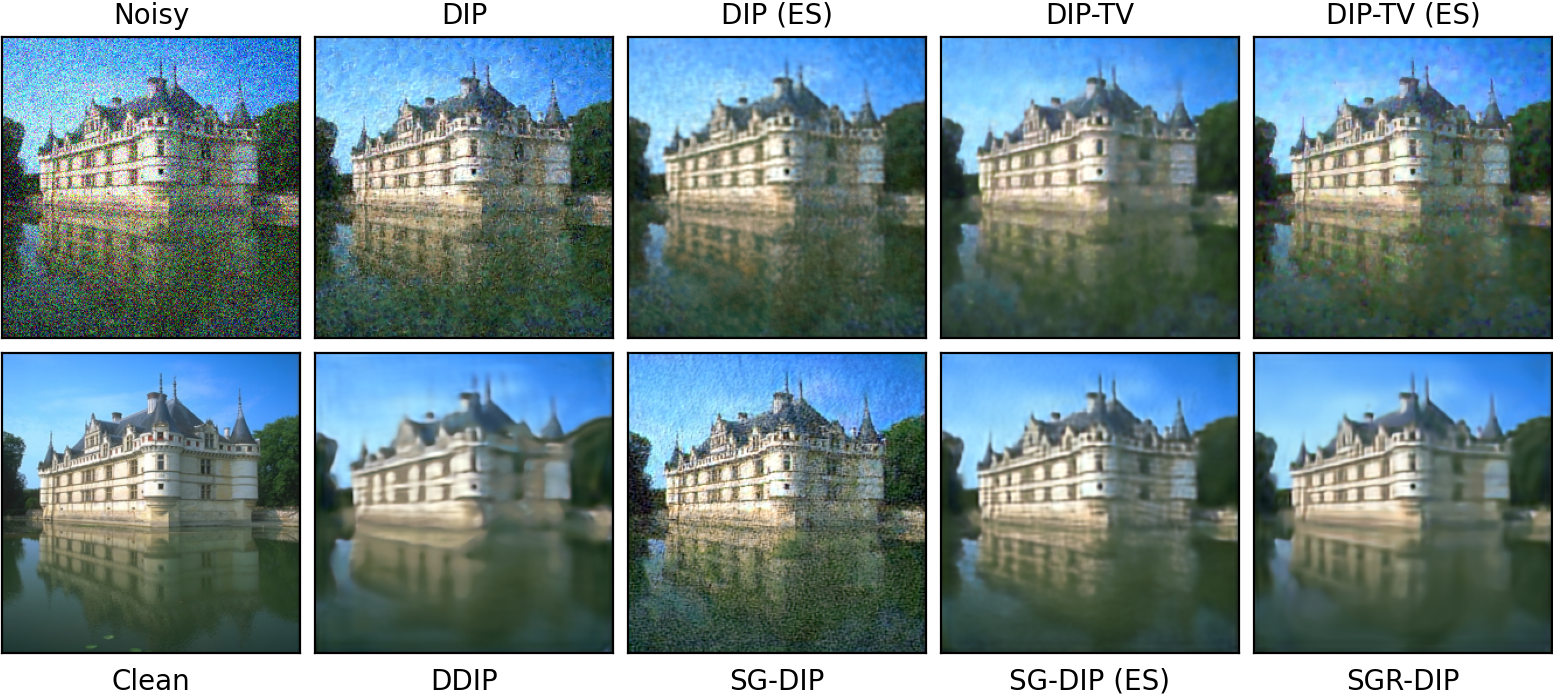
\includegraphics[width=\textwidth]{img/fig_6.2_1.png}\\
    \vspace{20pt}
    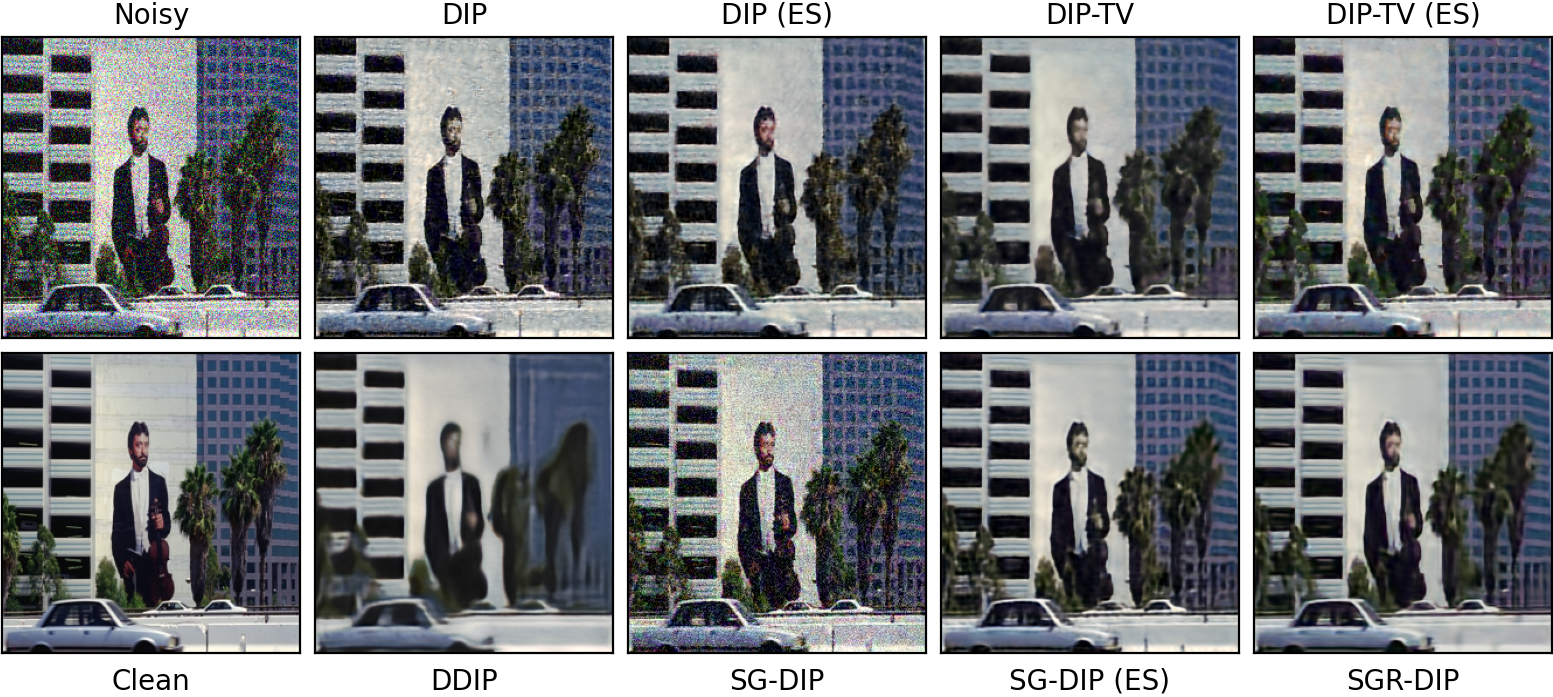
\includegraphics[width=\textwidth]{img/fig_6.2_2.png}
    \caption{
        Visual comparison of DIP variants on the CBSD68 dataset.
        Noisy input images are generated at a PSNR of 15\,dB.
    }\label{fig:CBSD68}
\end{figure}

\section{Distributed Acoustic Sensing Data}

For real-world DAS data, no clean reference data is available.
Consequently, evaluation primarily relies on visual comparison of denoised outputs and their residuals.
Additionally, we also consider the notion of local waveform coherence discussed in Section~\ref{sec:CC}.

We compare the DIP-based approaches with two other zero-shot denoising methods, namely BM3D~\cite{BM3D} and the integrated denoising framework (IDF) proposed by Chen et al.~\cite{IDF}.
Following~\cite{SelfMixed}, we set the noise standard deviation to 0.1 for BM3D and use the default parameters for IDF\@.

Our results indicate that findings from standard image denoising do not directly translate to DAS data.
While early-stopping strategies perform well for image data, ES-WMV proves inconsistent in DAS settings, as the variance curve often lacks a clear U-shape.
This often leads to stopping points either at the beginning or near the end of training.
Similarly, DIP-TV exhibits high sensitivity to the balancing parameter $\lambda$, with large values producing all-zero regions and small values reducing the regularization effect.
No single $\lambda$ value generalizes well across different signal intensities and varying DAS setups, making DIP-TV unsuitable as a general-purpose approach.
A similar issue arises with DDIP, where the regularization induced by the diffusion process is overly strong, typically resulting in all-zero outputs for DAS data.
These common failure modes are visualized in~\ref{fig:failure-cases}.

Out of the methods discussed so far, IDF, DIP and SGR-DIP yield the most promising results.
For the band-pass preprocessing of FORGE data, we use a high-cut frequency of 200\,Hz, following~\cite{IDF}.
For DIP, we decrease the maximum number of iterations to 1000, for SGR-DIP we set it to only 300.
Figure~\ref{fig:FORGE} provides a detailed comparison of these approaches on DAS samples with varying signal intensities (\textit{FORGE 1--3}, see Table~\ref{tab:sample-details}).

\begin{figure}[b!]
    \centering
    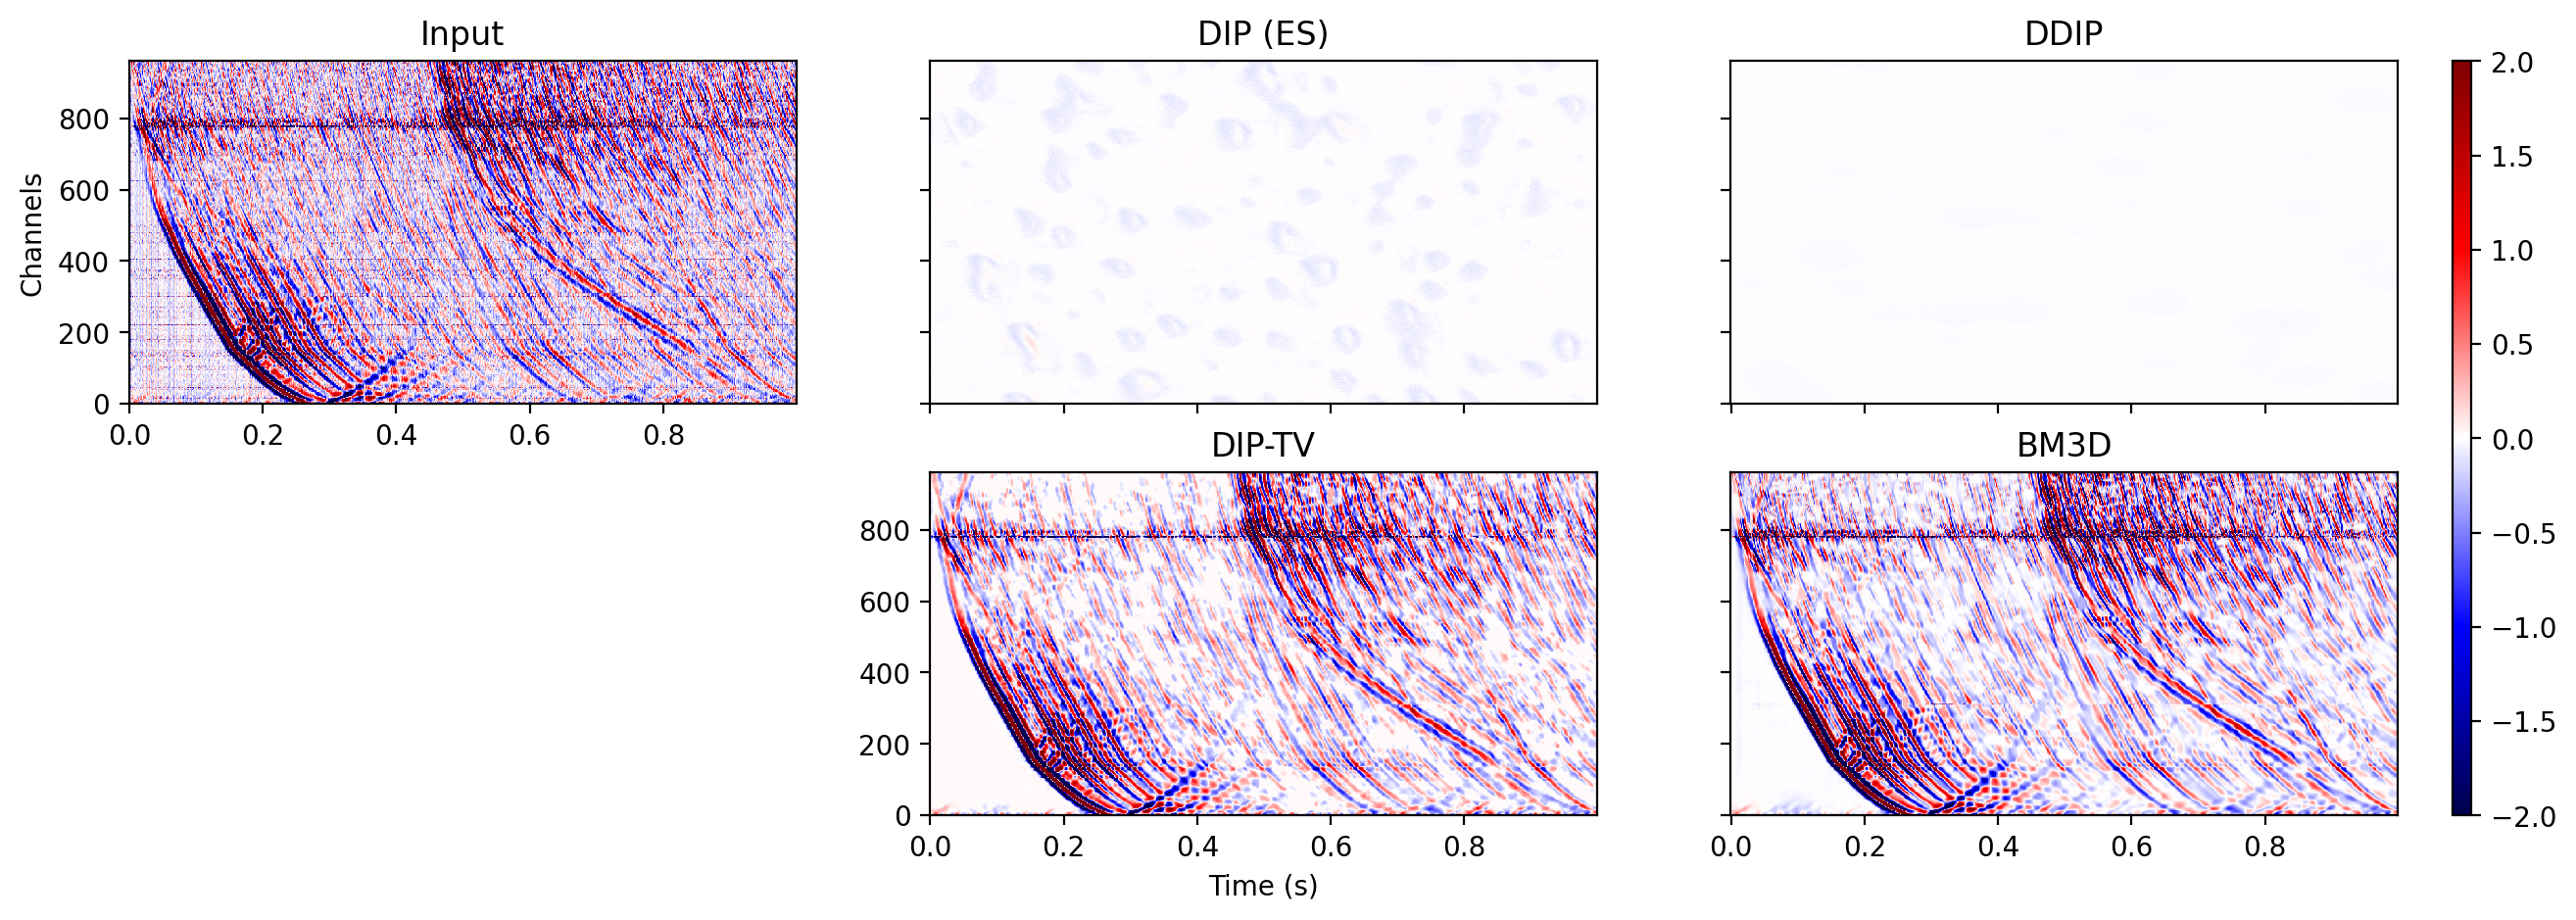
\includegraphics[width=\textwidth]{img/fig_6.3.png}
    \caption{
        Common failure modes of different denoising methods on the \textit{FORGE 1} sample.
        The detected optimal stopping point occurs too early in the training process and DDIP's regularization is too strong, both leading to an (almost) all-zero output.
        While DIP-TV and BM3D capture the signal, both methods produce regions of all-zero values.
        The noisy input is normalized by its standard deviation prior to denoising.
    }\label{fig:failure-cases}
\end{figure}


% XXX improve figure layout (fix spacing)
\begin{figure}
    \centering
    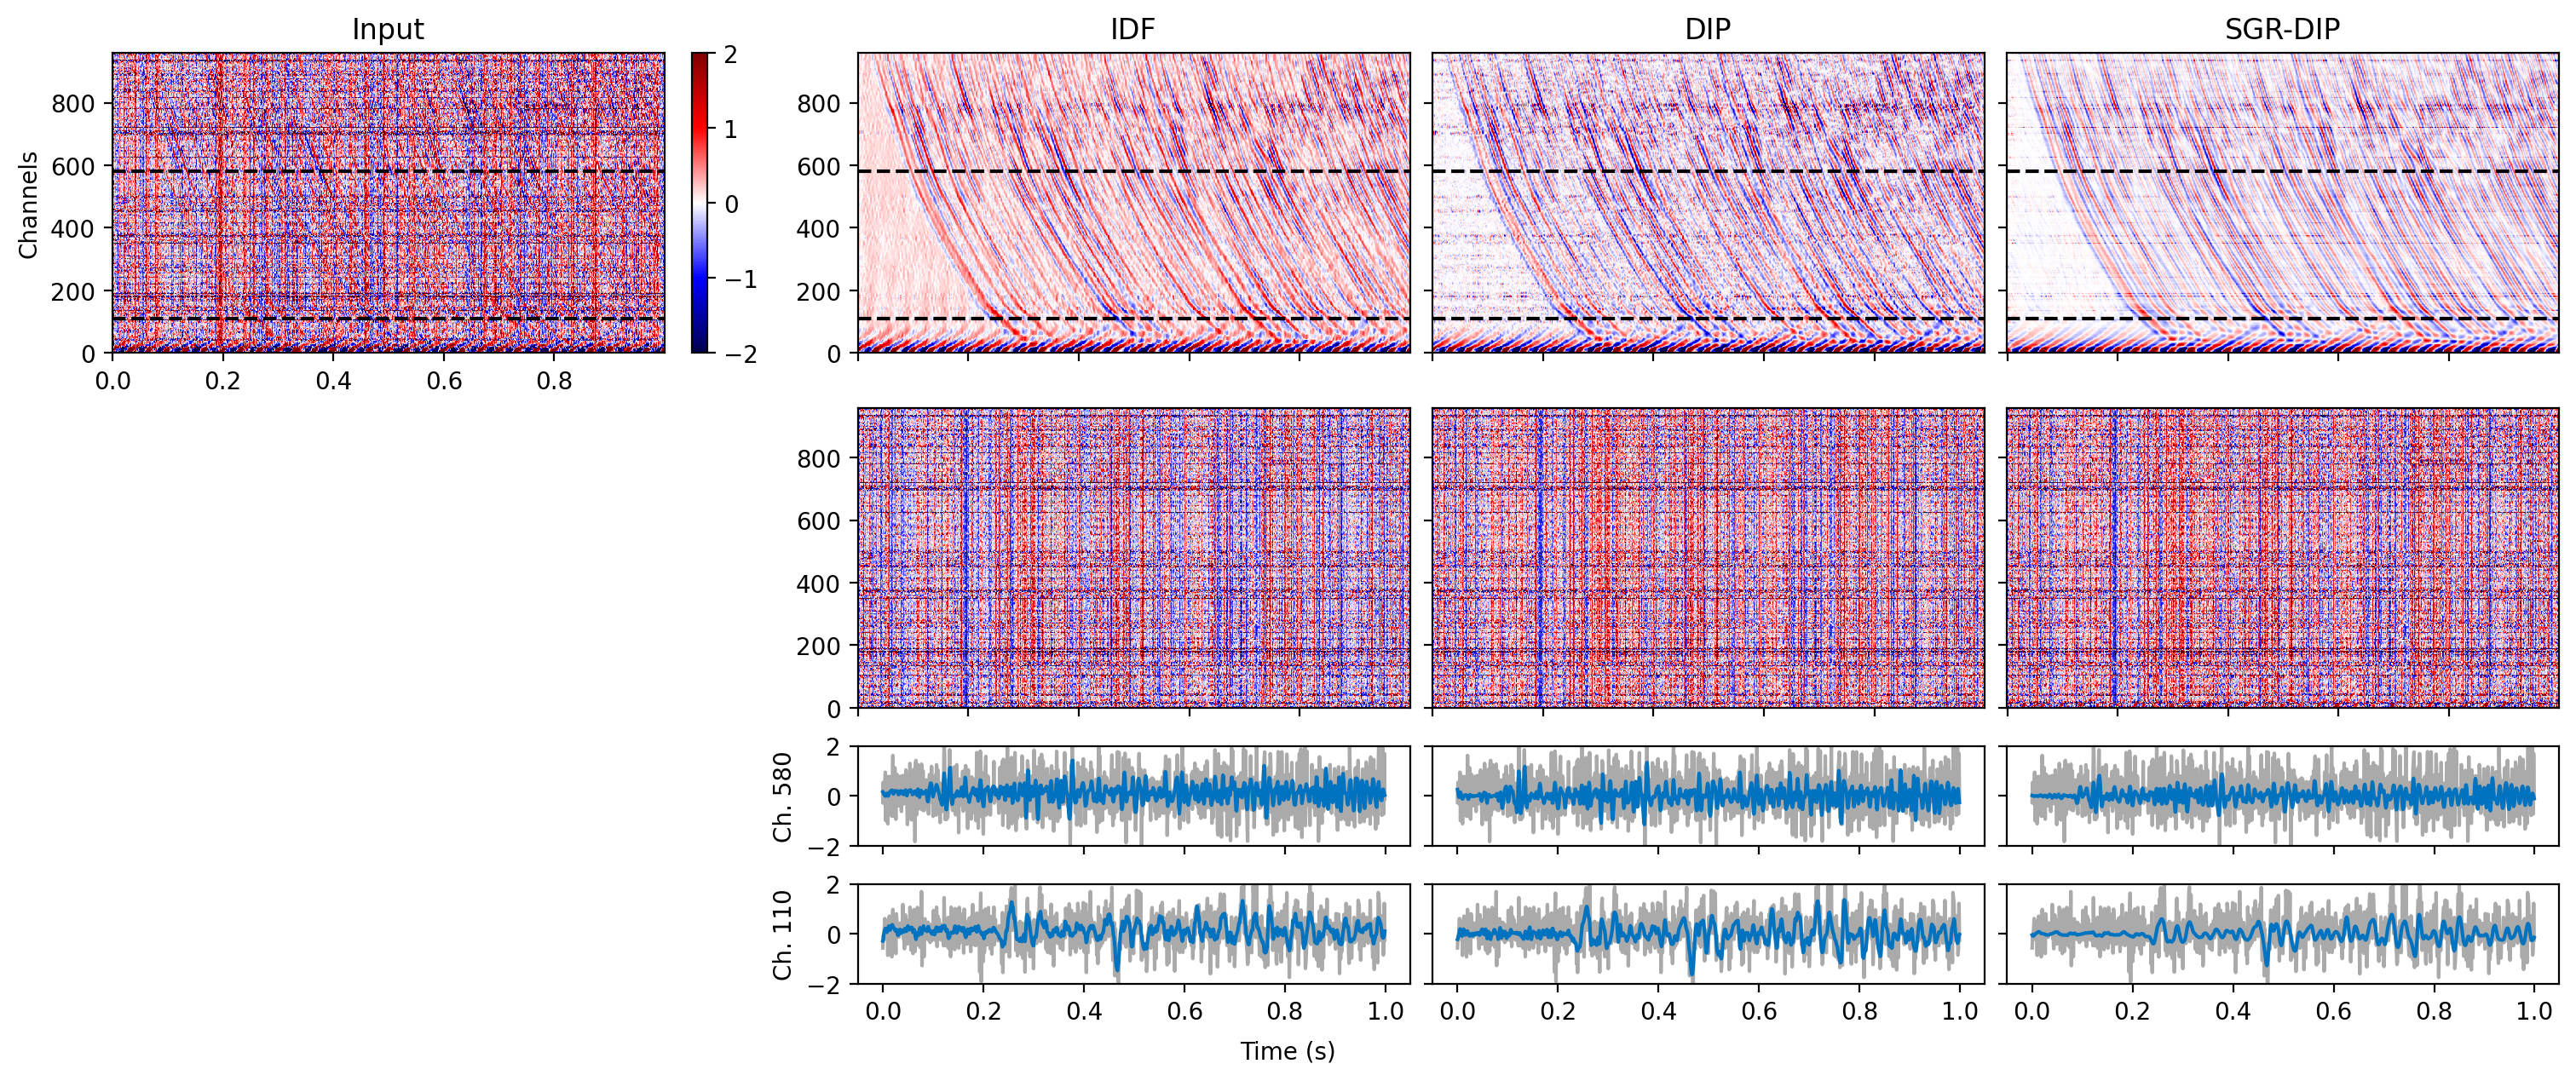
\includegraphics[width=\textwidth]{img/fig_6.4_1.png}\\
    \vspace{10pt}
    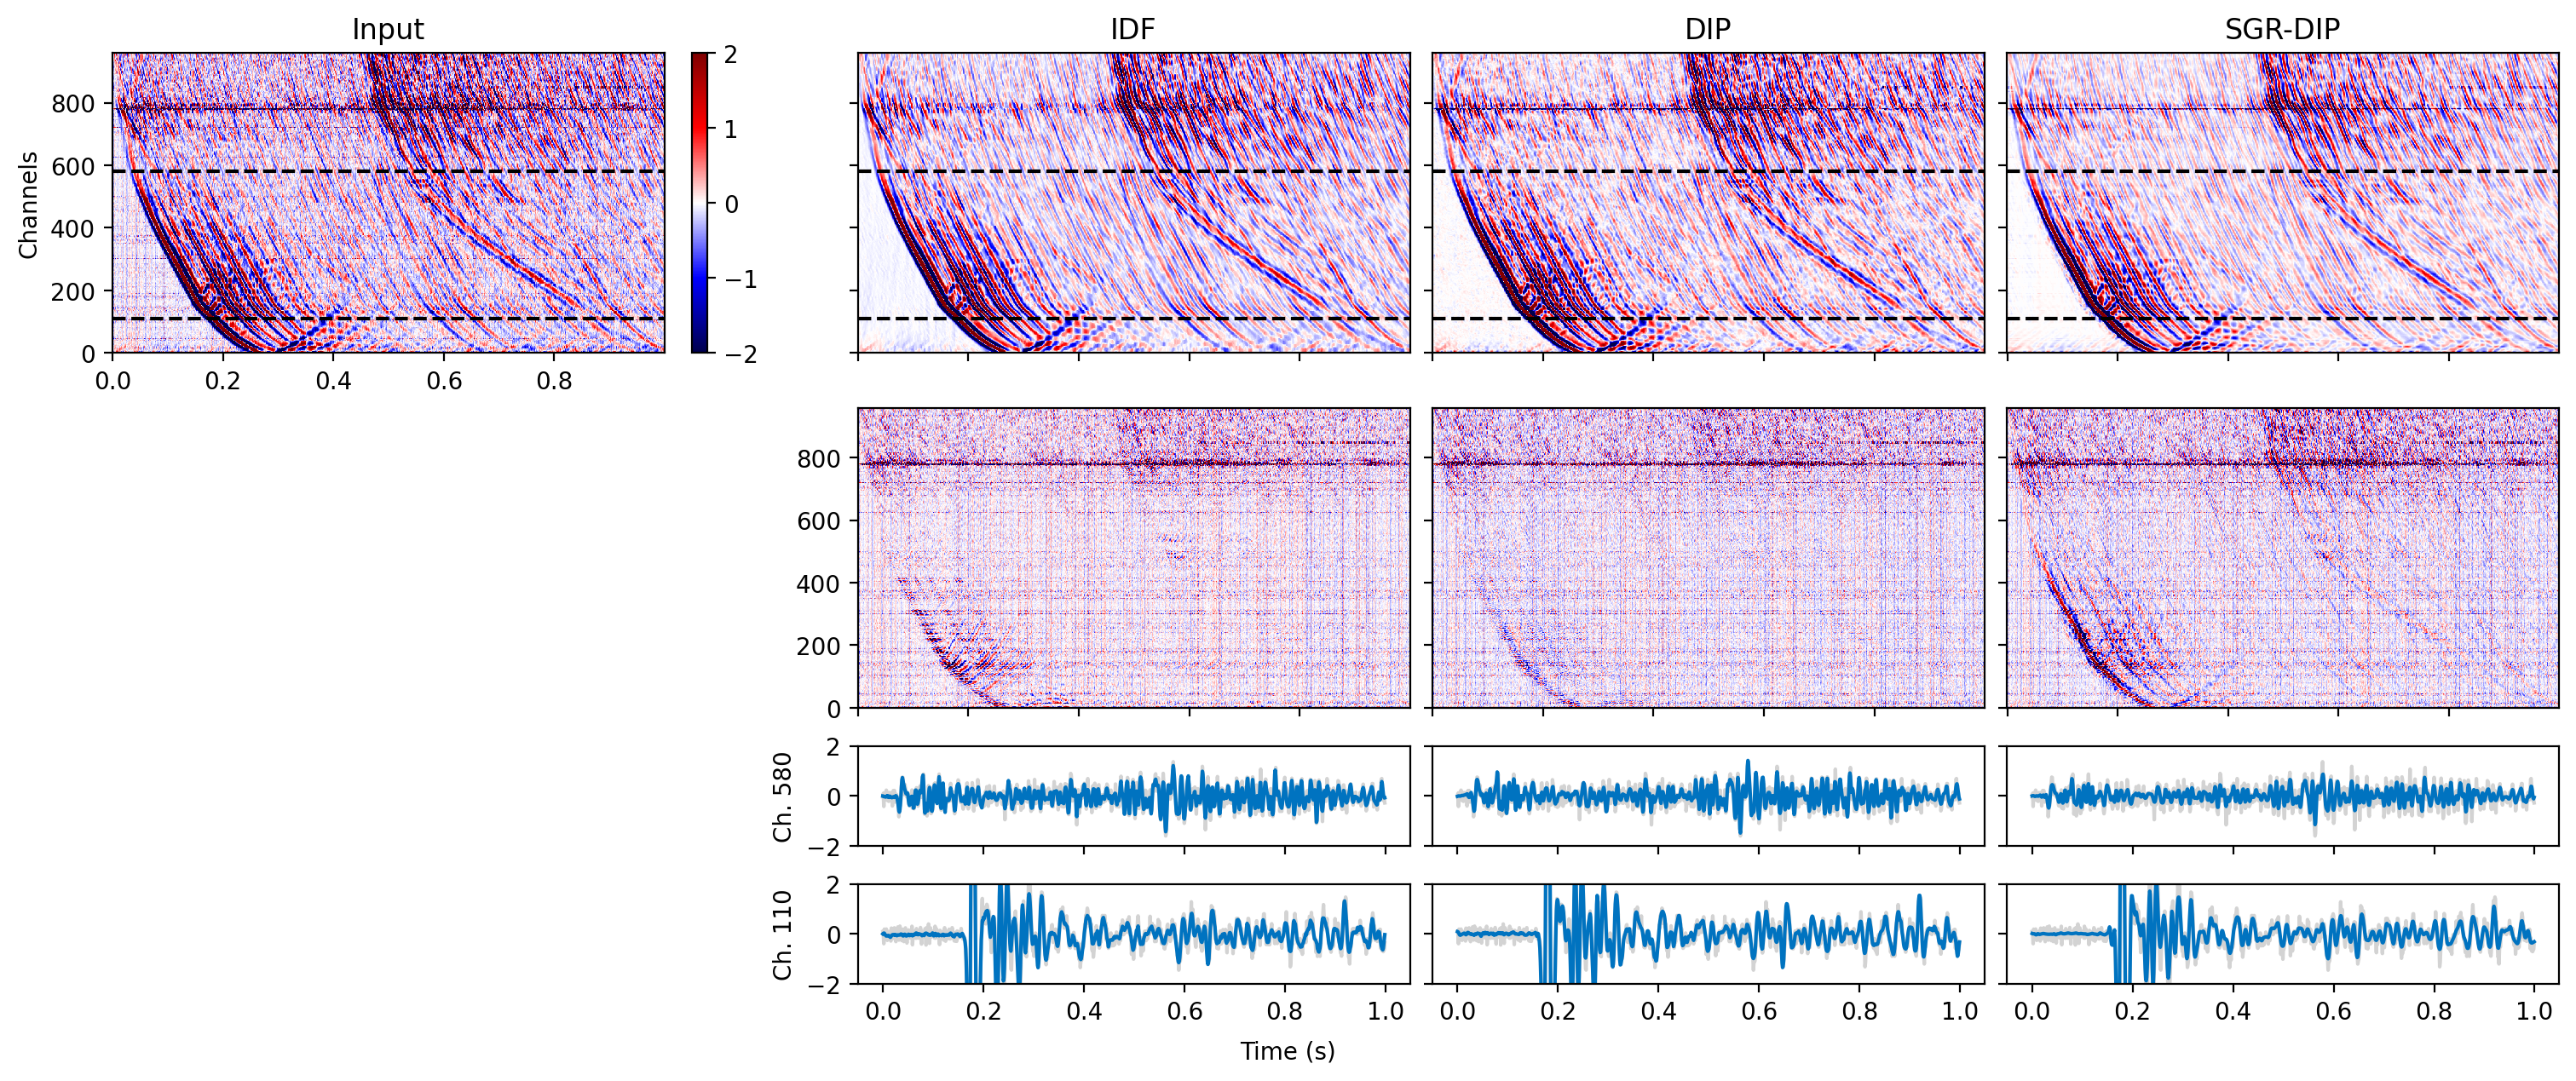
\includegraphics[width=\textwidth]{img/fig_6.4_2.png}\\
    \vspace{10pt}
    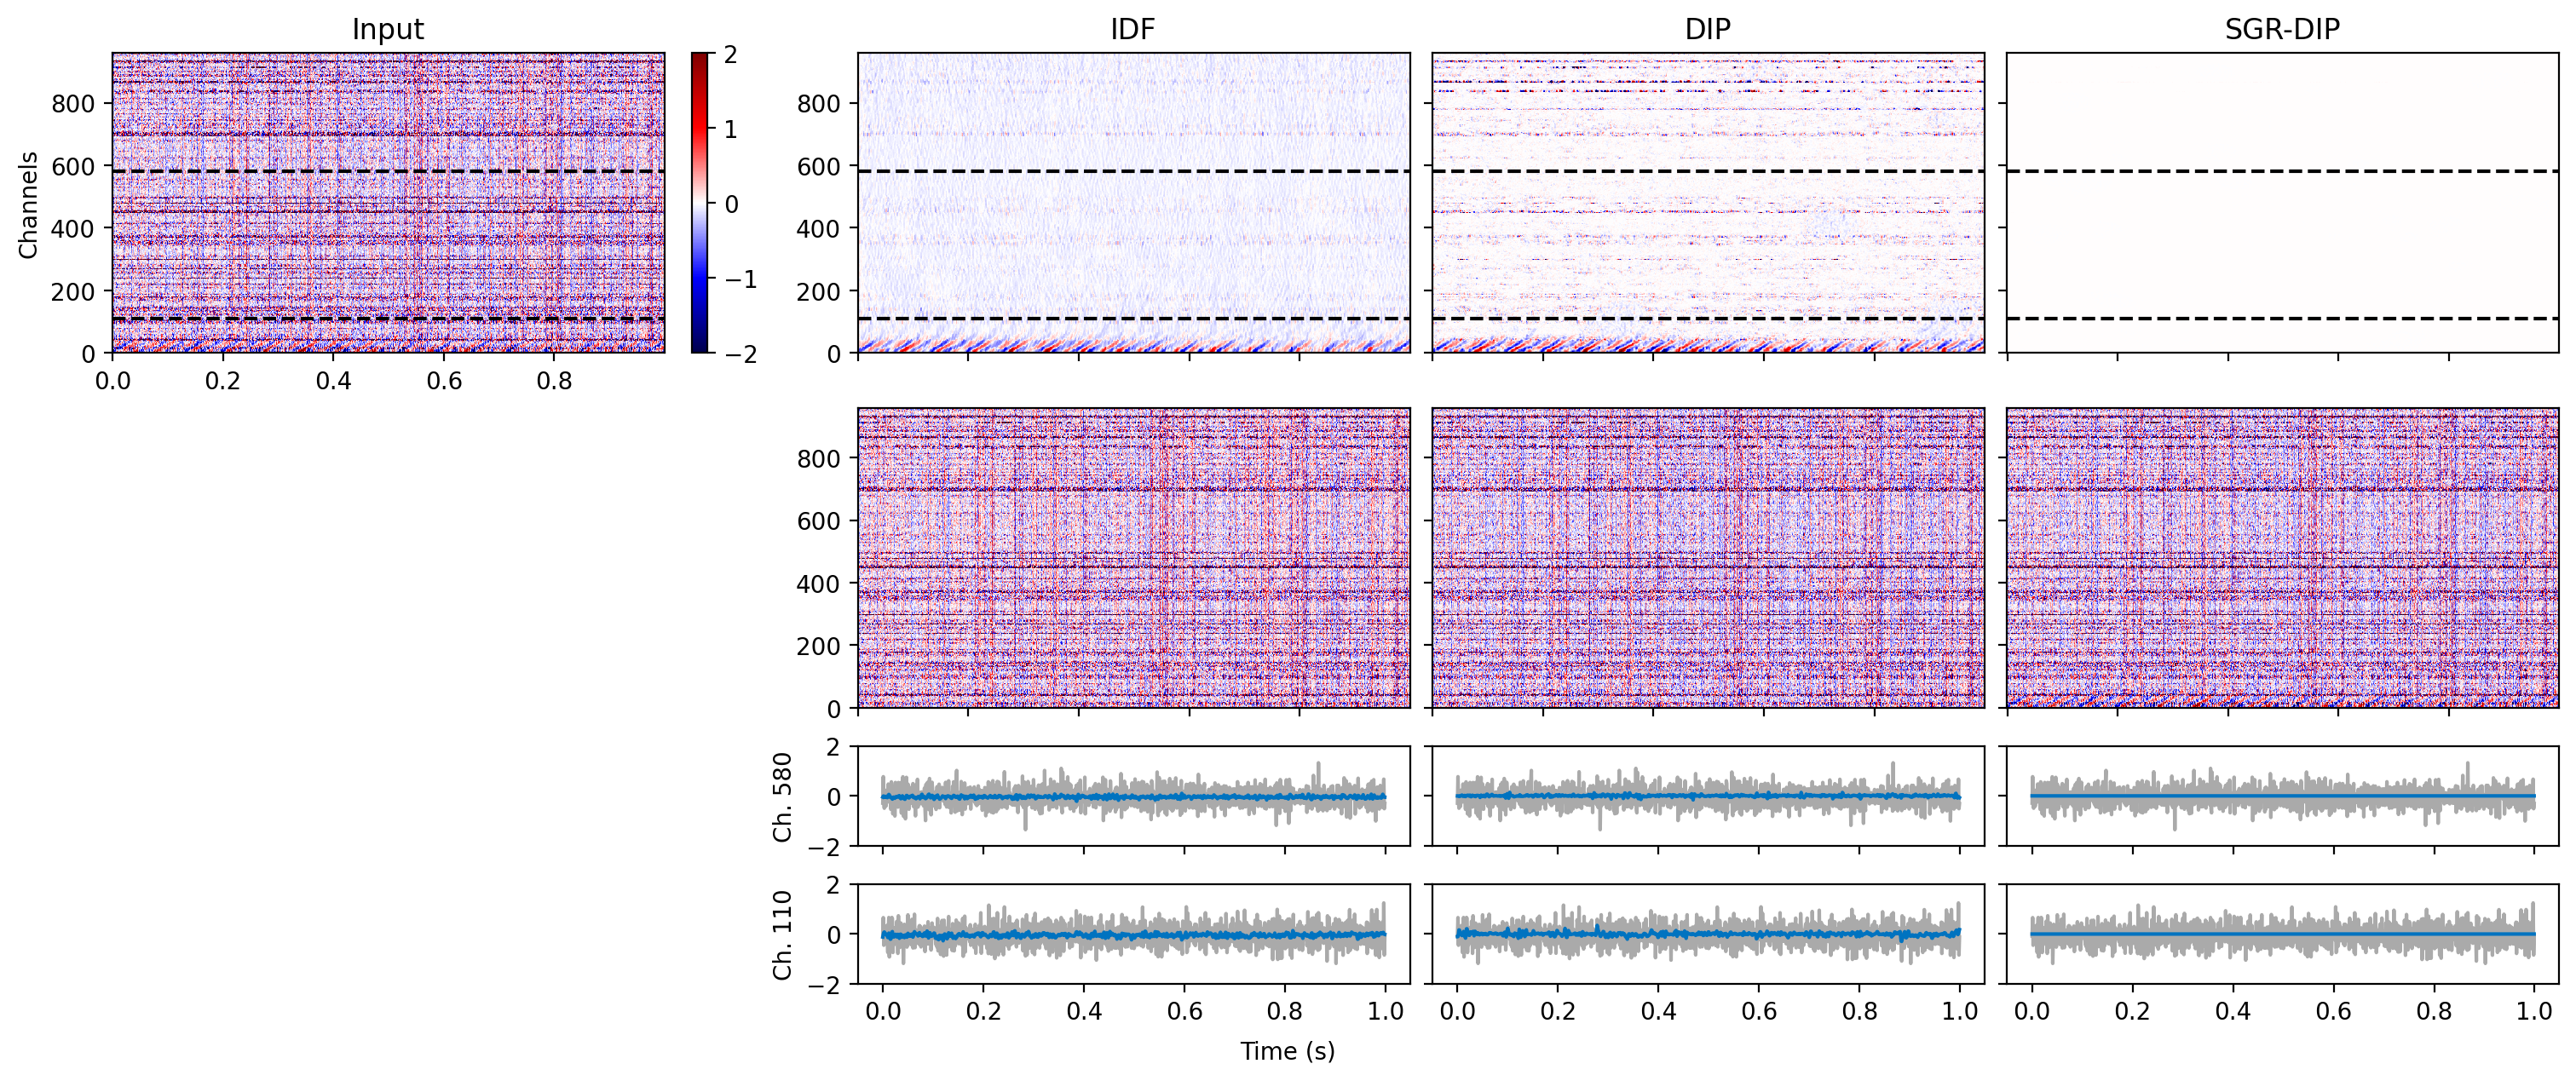
\includegraphics[width=\textwidth]{img/fig_6.4_3.png}
    \caption{
        Visual comparison of IDF, DIP, and SGR-DIP on 3 different DAS samples.
        The first two samples include moderately strong and strong signals, respectively; the last consists of pure noise.
        The first two rows show denoised results and the corresponding residuals.
        The third row provides measurements for individual channels indicated by the dashed black lines, gray curves represent the corresponding noisy channels.
        Noisy inputs are normalized by their standard deviation prior to denoising.
        Figure adapted from~\cite{DAS-CN2S}.
    }\label{fig:FORGE}
\end{figure}

\begin{figure}
    \centering
    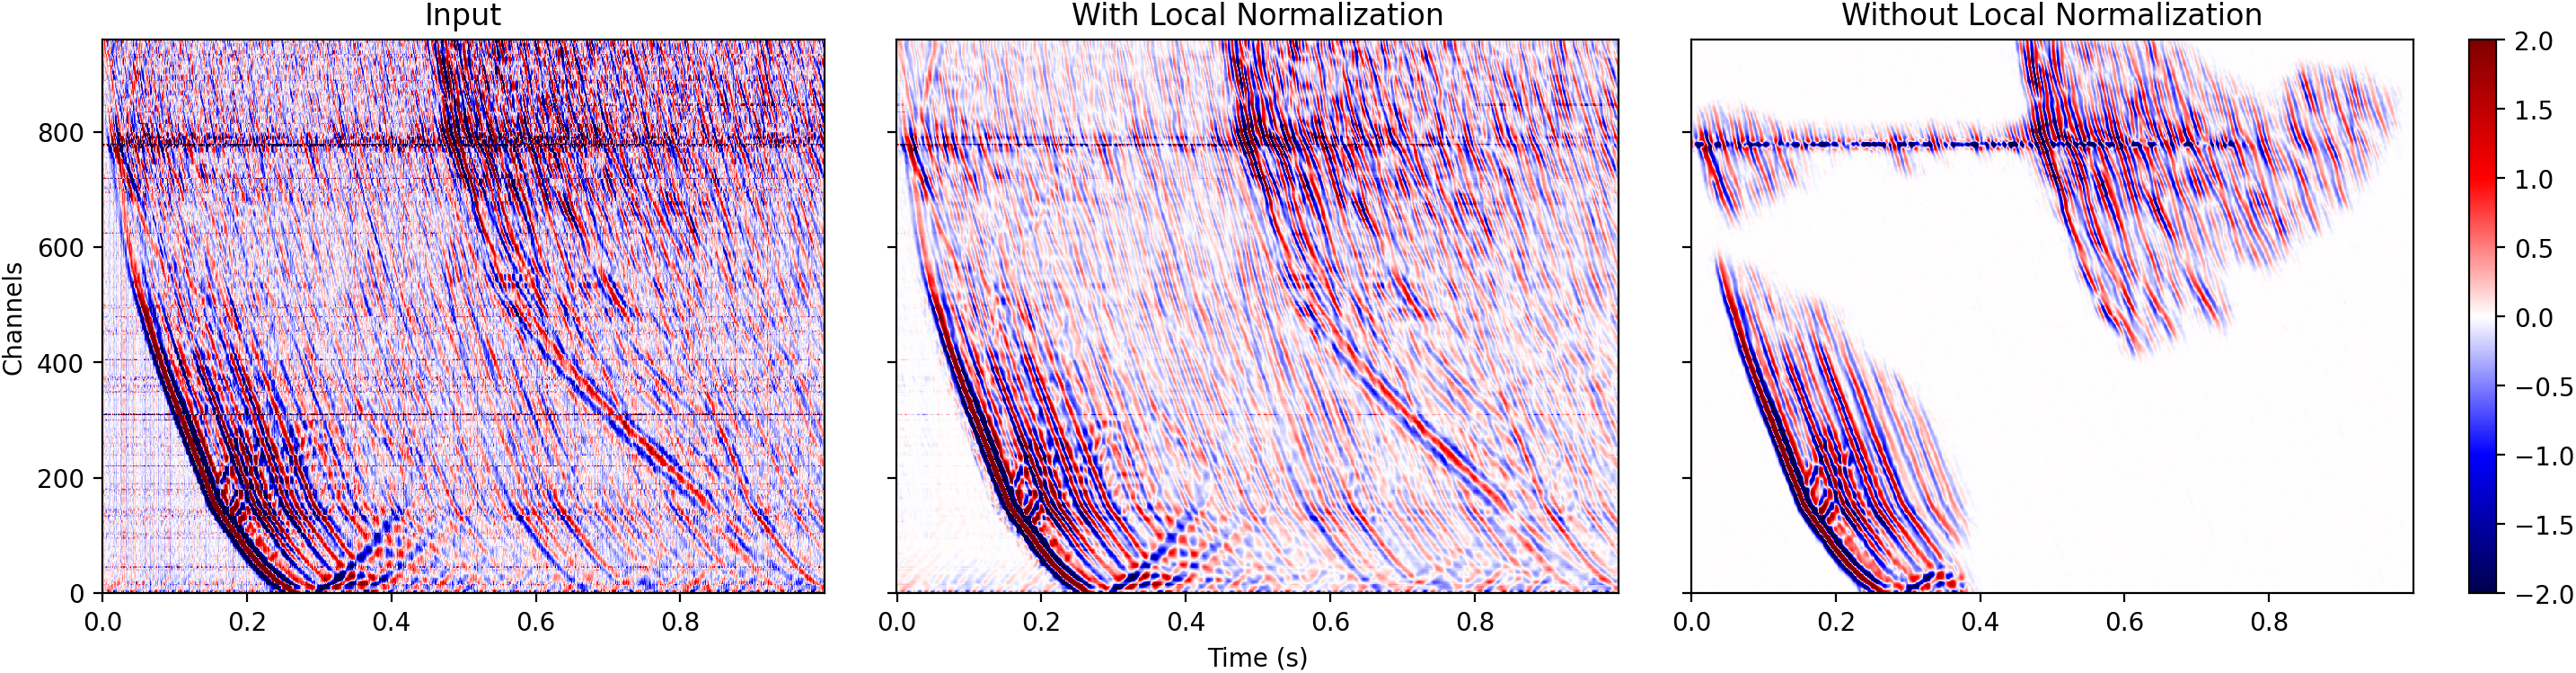
\includegraphics[width=\textwidth]{img/fig_6.5.png}
    \caption{
        Comparison of SGR-DIP with and without local normalization on the \textit{FORGE 1} sample.
        The noisy input is normalized by its standard deviation prior to denoising.
    }\label{fig:local-normalization}
\end{figure}

\begin{wraptable}{r}{0.48\textwidth}
    \centering
    \begin{tabular}{ l c }
        \toprule
        Method &Runtime (m) $\downarrow$\\
        \midrule
        IDF &0.12\\
        DIP &1.98\\
        SGR-DIP &1.94\\
        \bottomrule
    \end{tabular}
    \caption{Average runtimes of the methods visualized in Figure~\ref{fig:FORGE}.}\label{tab:runtimes}
\end{wraptable}

IDF demonstrates consistent performance across all signal intensities.
While DIP preserves more signal in the strong signal sample, outperforming IDF in this case, its performance slightly declines for lower signal intensities.
SGR-DIP surpasses both methods for moderately strong signals and is the only approach that correctly produces an all-zero output for the pure-noise sample.
However, it struggles to reproduce very high amplitudes, leading to greater signal loss in the strong signal case.

Another key consideration is runtime.
Unlike DIP and SGR-DIP, which require training an entire neural network, the DL-free IDF is significantly faster, as detailed in Table~\ref{tab:runtimes}.
A notable observation is the differing impact of local normalization on the DIP-based methods. 
While it slightly degrades denoising performance in DIP, it is essential for SGR-DIP, as illustrated in Figure~\ref{fig:local-normalization}.

In addition to the FORGE dataset, we conduct experiments on data recorded during the SISSLE experiment.
For band-pass preprocessing, we use a high-cut frequency of 10\,Hz, following~\cite{DAS-CN2S}.
As before, we compare IDF, DIP, and SGR-DIP\@.
For SGR-DIP, we use the modification where the noisy sample serves as the initial $z$ and set the noise standard deviation $\sigma = \frac{3\max(z)}{4}$, as discussed in Section~\ref{sec:SG-DIP}.

All three methods enhance local waveform coherence; however, they also attenuate the P- and S-waves of the earthquake present in the sample.
To mitigate this issue, we investigate omitting the band-pass preprocessing.
While this leads to additional artifacts in SGR-DIP, it allows DIP to better preserve the P-wave while still suppressing incoherent noise.
However, in this case, the improvement in local waveform coherence is only marginal compared to the noisy input. 
Both variants are visualized in Figure~\ref{fig:SISSLE}.

\begin{figure}
    \centering
    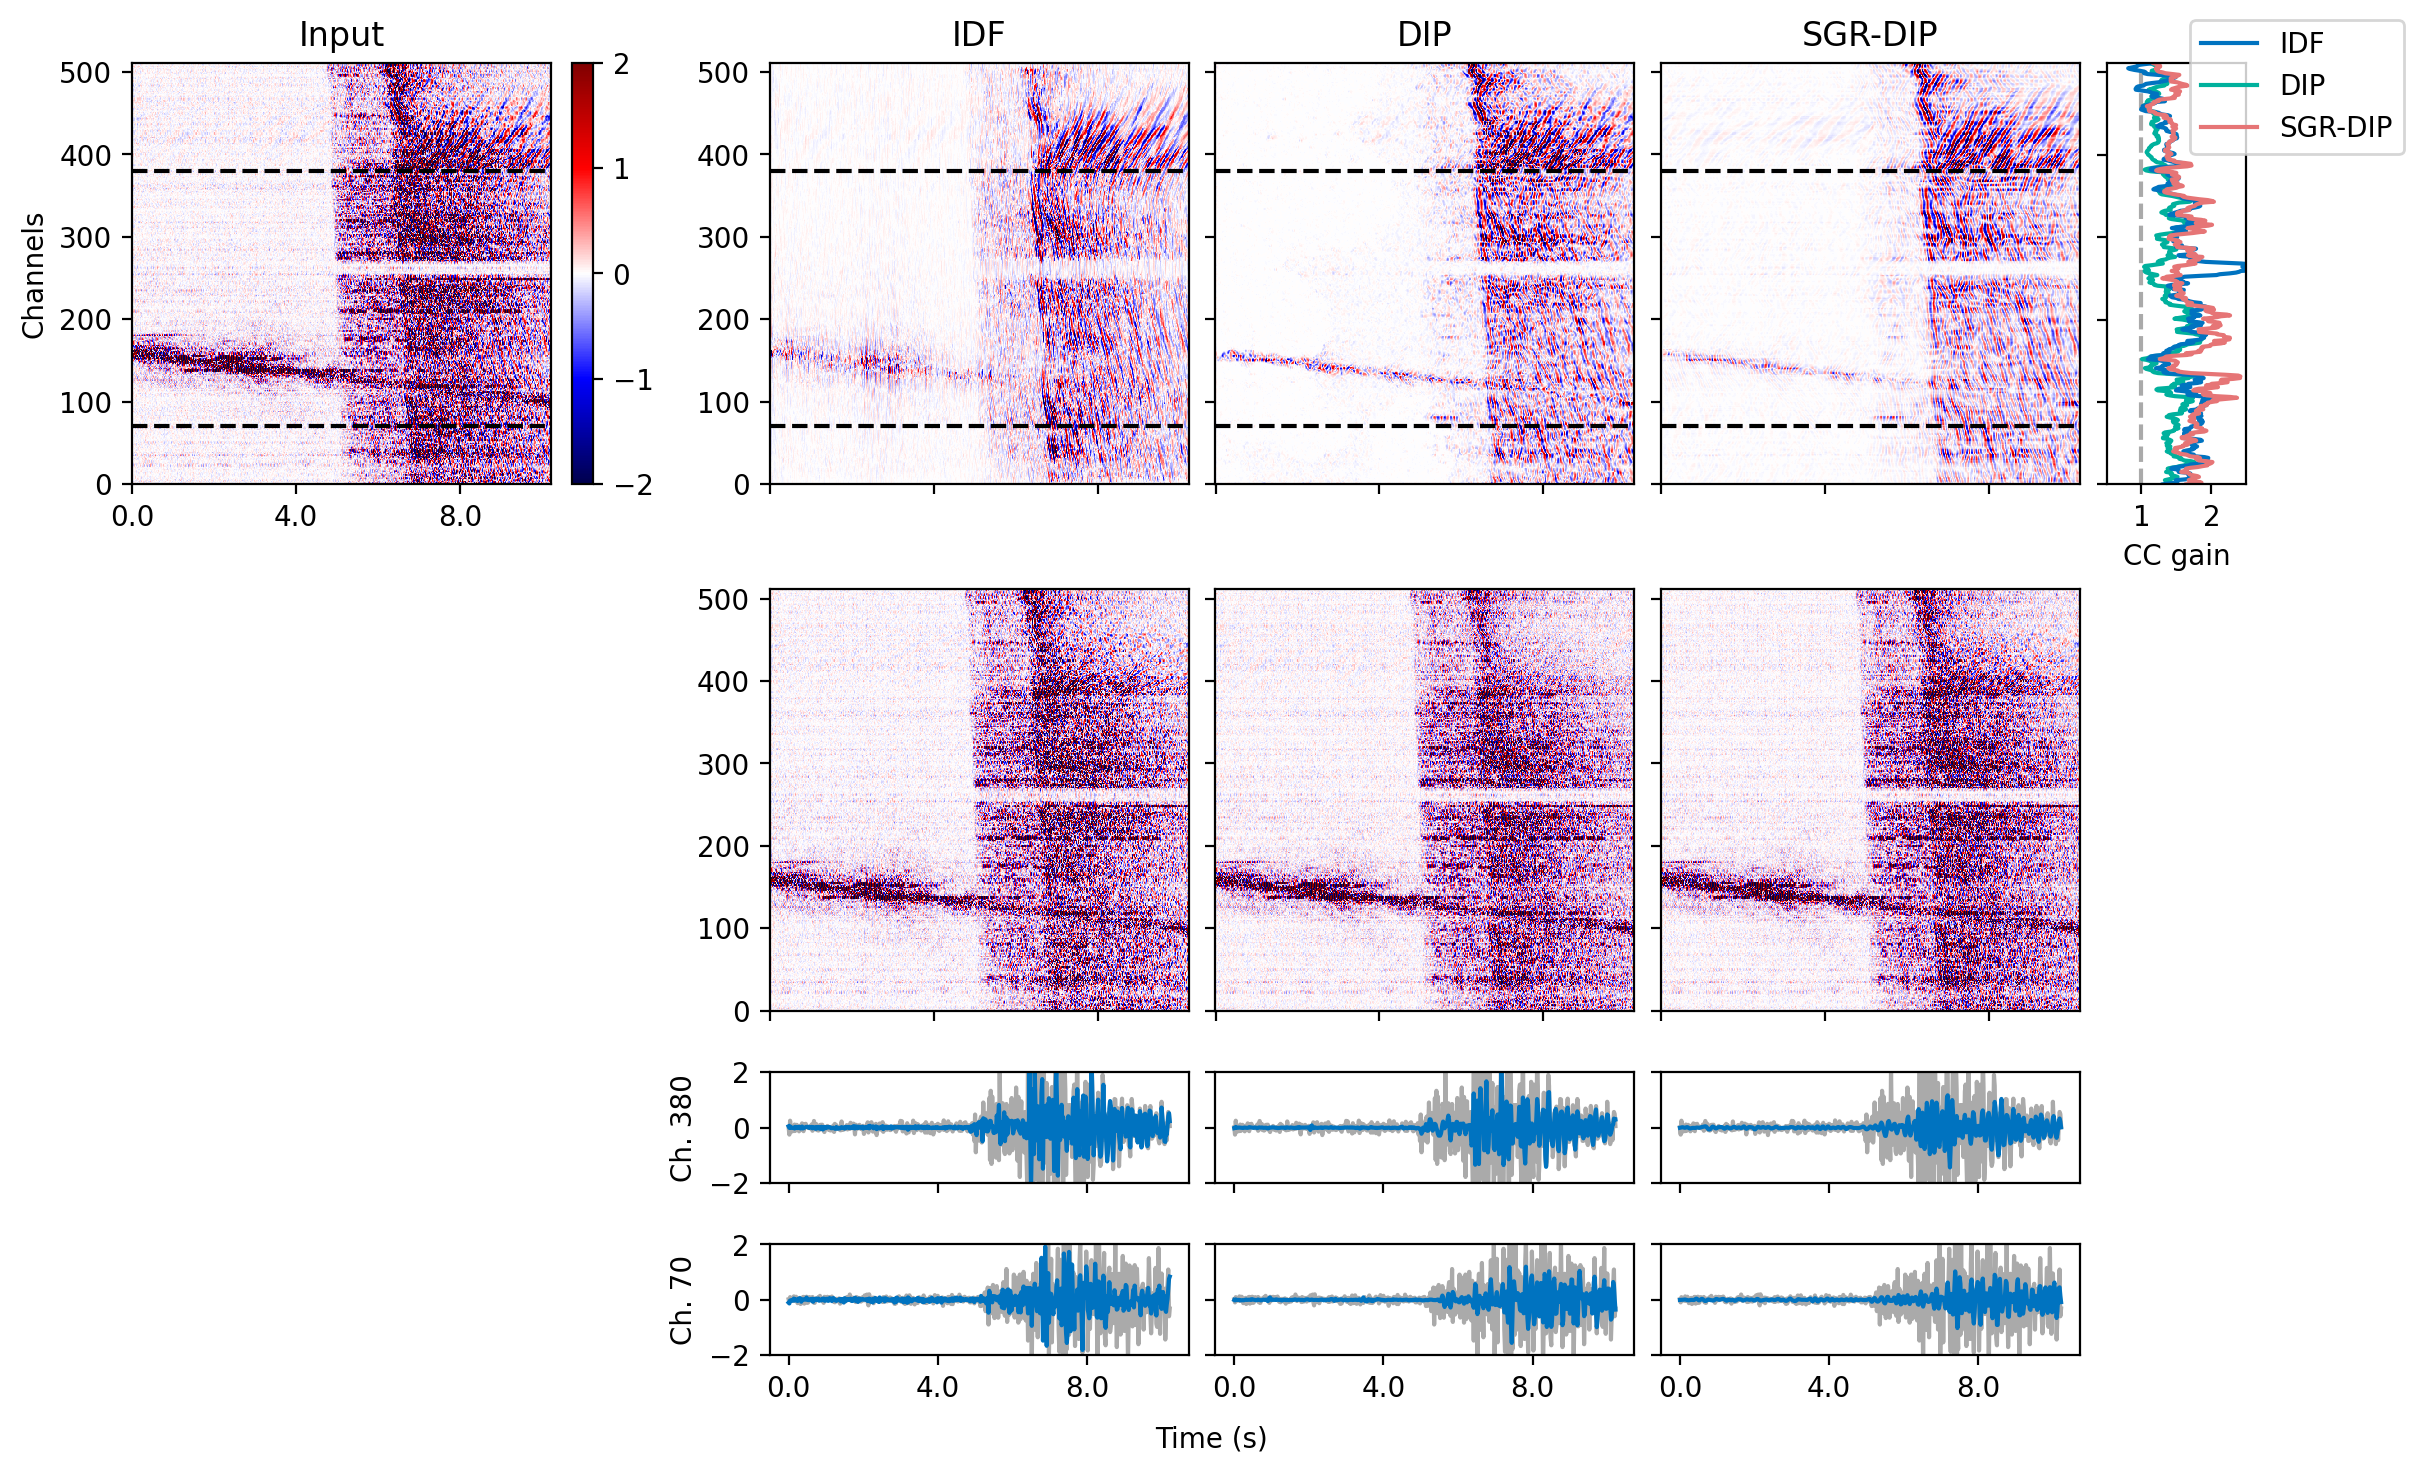
\includegraphics[width=\textwidth]{img/fig_6.6_1.png}\\
    \vspace{10pt}
    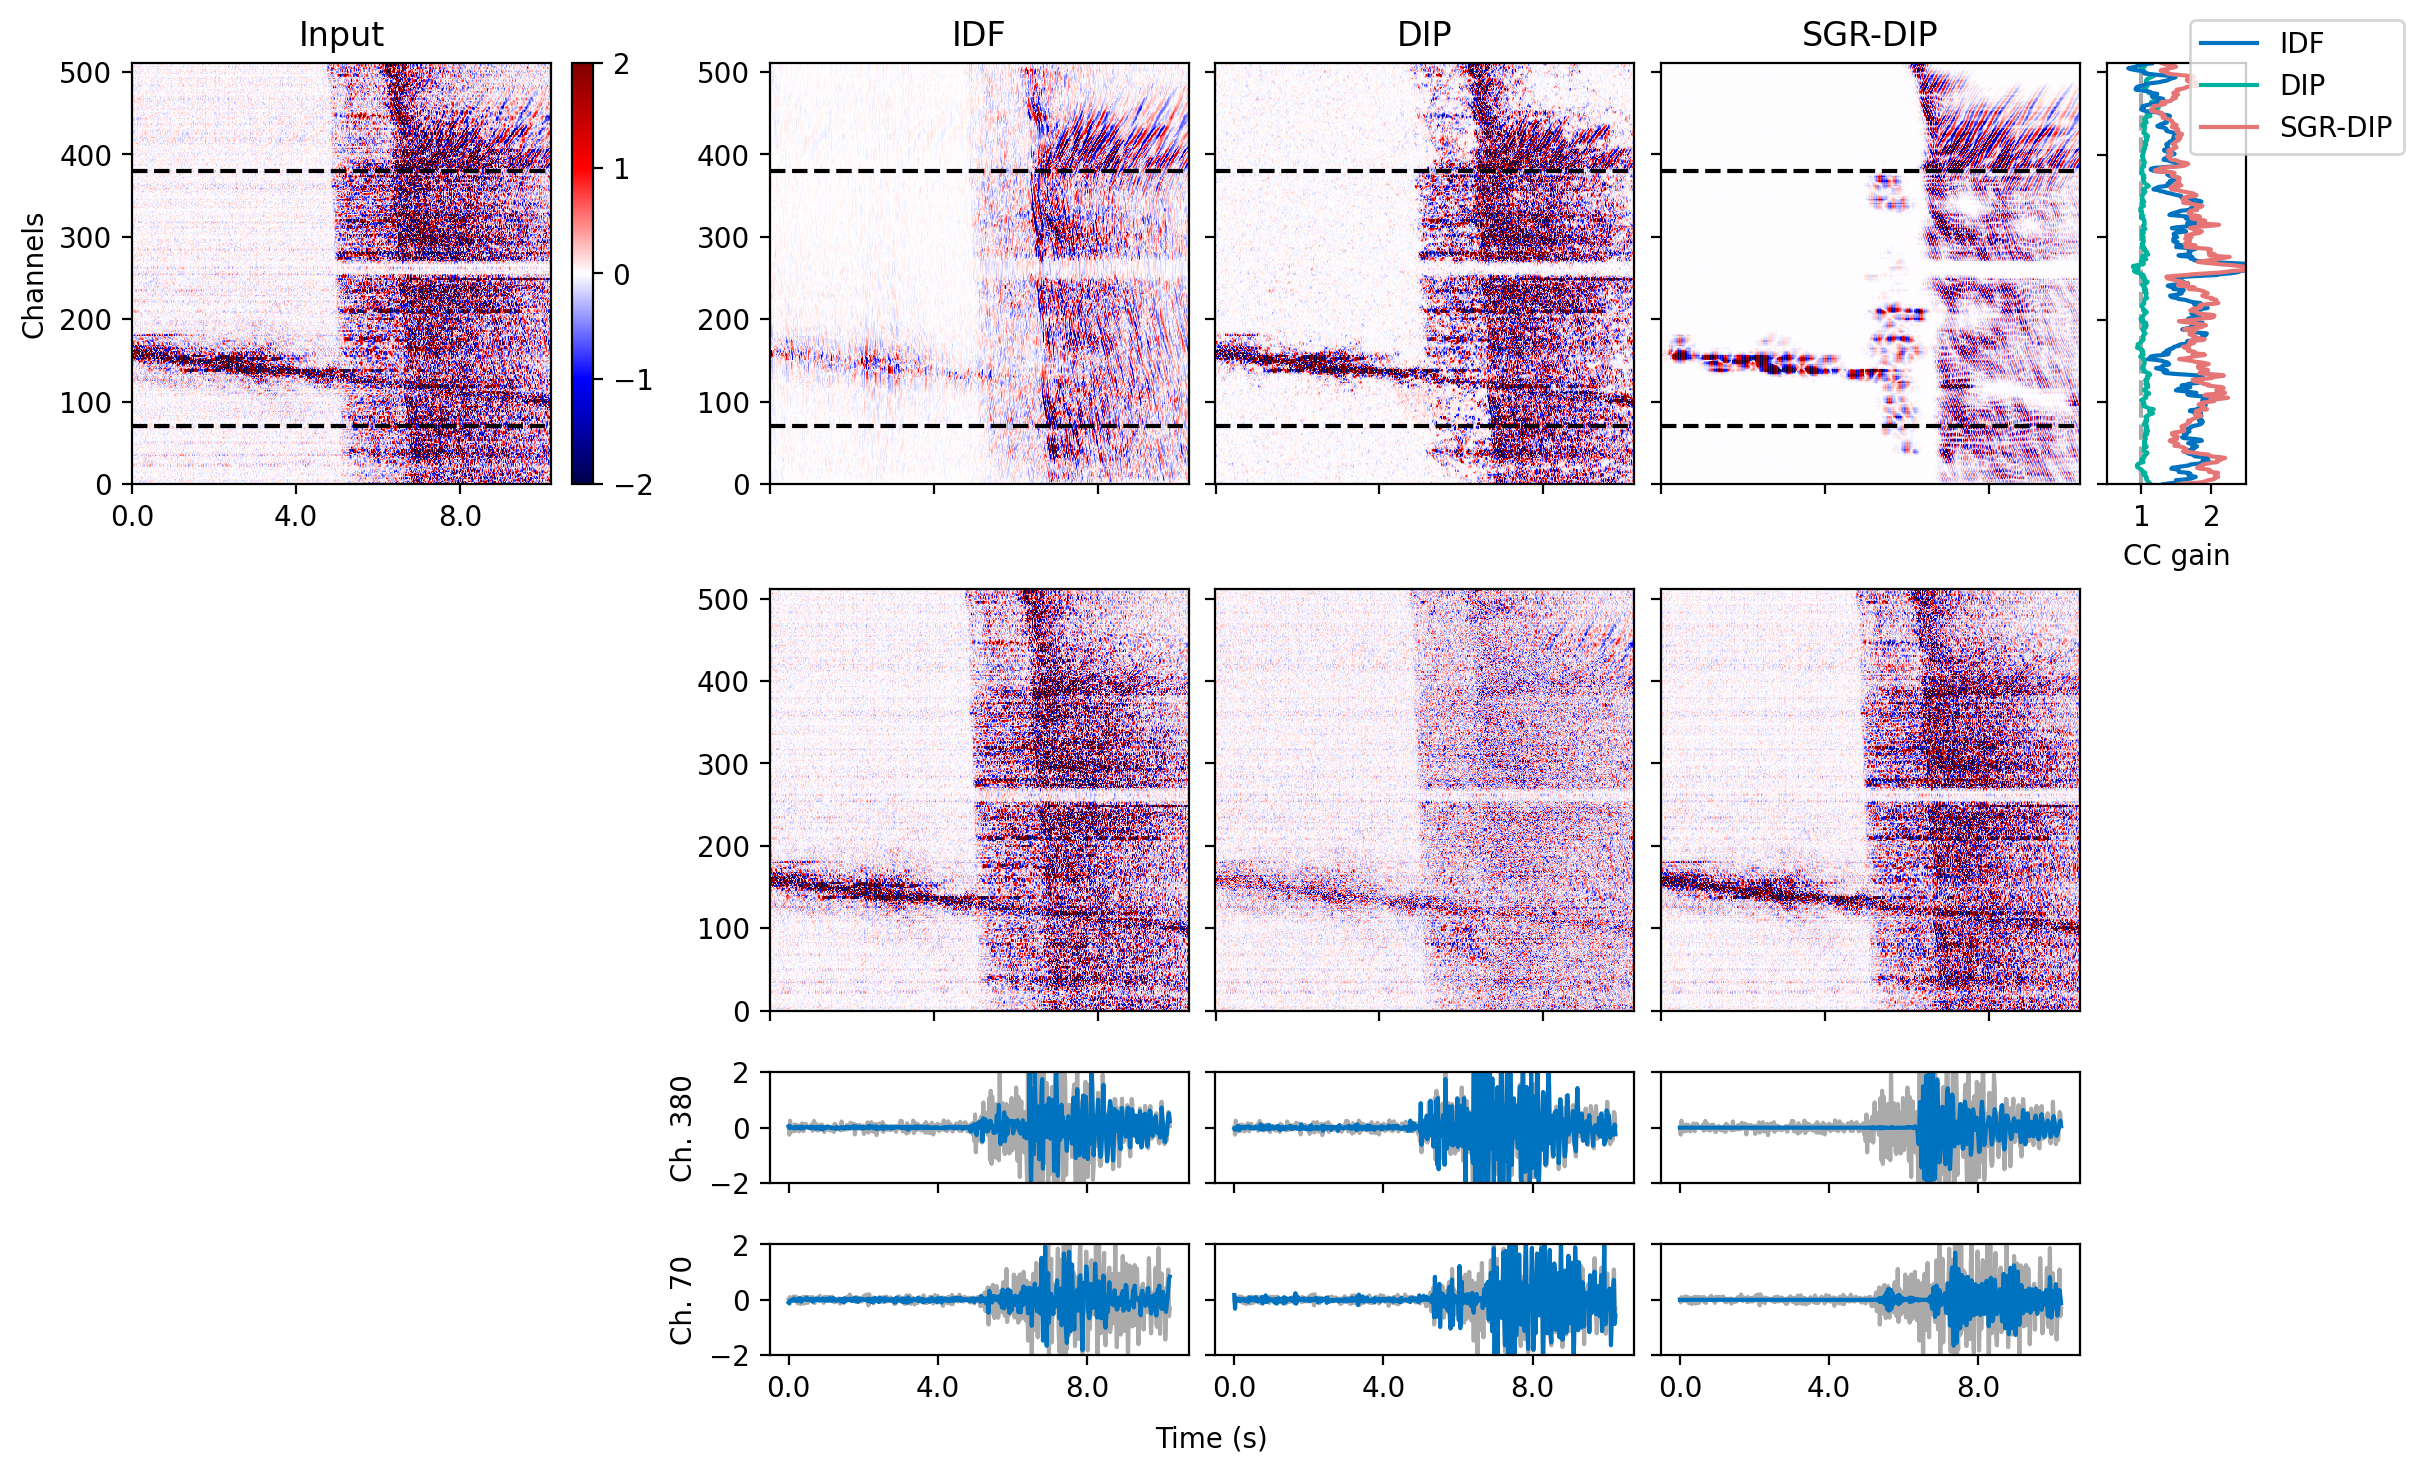
\includegraphics[width=\textwidth]{img/fig_6.6_2.png}
    \caption{
        Visual comparison of IDF, DIP, and SGR-DIP on the \textit{SISSLE 1} sample with and without band-pass preprocessing.
        Note that the input and IDF results are identical in both cases and are only given for easier reference.
        The first two rows show denoised results and the corresponding residuals.
        The third row provides measurements for individual channels indicated by the dashed black lines, gray curves represent the corresponding noisy channels.
        Noisy inputs are normalized by their standard deviation prior to denoising.
        Figure adapted from~\cite{DAS-CN2S}.
    }\label{fig:SISSLE}
\end{figure}
